\documentclass[a4paper, 10pt,notumble]{leaflet}
%Adjust paragraph indentation.
\setlength{\parindent}{0pt}
\setlength{\belowcaptionskip}{-20pt}
\usepackage{printlen}

% Diagram for cover art
\usepackage{tikz}
\usetikzlibrary{shapes}
\usetikzlibrary{patterns}

\usepackage{caption}
\usepackage{array}
\usepackage{booktabs}

\usepackage[type={CC}, version={4.0}, modifier={by}]{doclicense} % Add text and icons for creative commons license

% Adjust formatting of list environments
\usepackage{enumitem}
\usepackage{calc}
\usepackage{multicol}

\setlist[itemize]{noitemsep, topsep=0pt, leftmargin=0.75cm, itemsep=\smallskipamount, labelindent=0.25cm}

\setlist[enumerate]{noitemsep, topsep=0pt, leftmargin=0.75cm, itemsep=\smallskipamount, labelindent=0.25cm}

\setlist[description]{noitemsep, topsep=0pt, labelindent=0.25cm, leftmargin=0.75cm, itemsep=\smallskipamount, font=\normalfont\bfseries}

\newlist{cardlist}{description}{1}
\newlist{playerlist}{description}{1}
\newlist{playerlistnarrow}{description}{1}
\newlist{personadecklist}{description}{1}
\newlist{auxiliarydecklist}{description}{1}
\newlist{challengetypelist}{description}{1}

\setlist[cardlist]{noitemsep, topsep=0pt, labelindent=0.25cm, leftmargin= 0.5cm,  labelsep=\widthof{\space}, font=\normalfont}

\setlist[playerlist]{noitemsep, topsep=0pt, labelindent=0.25cm, leftmargin= 0.5cm,  labelsep=\widthof{\space}, font=\normalfont, labelwidth=\widthof{\redace\diamonds\ (The Student):\ }}

\setlist[playerlistnarrow]{noitemsep, topsep=0pt, labelindent=0.25cm, leftmargin= 0.5cm,  labelsep=\widthof{\space}, font=\normalfont\bfseries, labelwidth=\widthof{The Student:\ }}

\setlist[personadecklist]{noitemsep, topsep=0pt, labelindent=0.25cm, leftmargin= 0.5cm,  labelsep=\widthof{\space}, font=\normalfont\bfseries, labelwidth=\widthof{\textbf{Voting\ Cards\ \ (16)}}}

\setlist[auxiliarydecklist]{noitemsep, topsep=0pt, labelindent=0.25cm, leftmargin= 0.5cm,  labelsep=\widthof{\space}, font=\normalfont\bfseries, labelwidth=\widthof{\textbf{Challenge\ Cards\ \ (27)}}}

\setlist[challengetypelist]{noitemsep, topsep=0pt, labelindent=0.25cm, leftmargin= 0.5cm,  labelsep=\widthof{\space}, font=\normalfont, labelwidth=\widthof{\clubs\ (Physcial):\ }}

% Setting Fonts
\usepackage{fontspec}
\renewfontfamily\sectfont[UprightFont={*-Black}]{Charter}

% Macros for symbols that appear on playing cards
\newfontfamily\cardfont{Card Characters}[Scale=1.0]

\DeclareRobustCommand\spades[1][black]{\textcolor{#1}{\cardfont{\}}}}
\DeclareRobustCommand\hearts[1][red]{\textcolor{#1}{{\cardfont{\{}}}}
\DeclareRobustCommand\diamonds[1][red]{\textcolor{#1}{{\cardfont{[}}}}
\DeclareRobustCommand\clubs[1][black]{\textcolor{#1}{\cardfont{]}}}

\DeclareRobustCommand\two[1][black]{\textcolor{#1}{\cardfont{2}}}
\DeclareRobustCommand\three[1][black]{\textcolor{#1}{\cardfont{3}}}
\DeclareRobustCommand\four[1][black]{\textcolor{#1}{\cardfont{4}}}
\DeclareRobustCommand\five[1][black]{\textcolor{#1}{\cardfont{5}}}
\DeclareRobustCommand\six[1][black]{\textcolor{#1}{\cardfont{6}}}
\DeclareRobustCommand\seven[1][black]{\textcolor{#1}{\cardfont{7}}}
\DeclareRobustCommand\eight[1][black]{\textcolor{#1}{\cardfont{8}}}
\DeclareRobustCommand\nine[1][black]{\textcolor{#1}{\cardfont{9}}}
\DeclareRobustCommand\ten[1][black]{\textcolor{#1}{\cardfont{=}}}

\DeclareRobustCommand\jack[1][black]{\textcolor{#1}{\cardfont{J}}}
\DeclareRobustCommand\queen[1][black]{\textcolor{#1}{\cardfont{Q}}}
\DeclareRobustCommand\king[1][black]{\textcolor{#1}{\cardfont{K}}}
\DeclareRobustCommand\ace[1][black]{\textcolor{#1}{\cardfont{A}}}
\DeclareRobustCommand{\joker}[1][black]{\begin{tikzpicture}[baseline=-0.4em]
	\path[draw, semithick, #1] (0,0) circle (1.5mm);
	\path[#1, draw, fill=#1, rounded corners=0.1mm] (90:1.45mm) to (234:1.45mm) to (18:1.45mm) to (162:1.45mm) to (306:1.45mm) to cycle;%
\path (-2mm, 0) to (0mm, 0);
\end{tikzpicture}}%


\DeclareRobustCommand\redtwo[1][red]{\textcolor{#1}{\cardfont{2}}}
\DeclareRobustCommand\redthree[1][red]{\textcolor{#1}{\cardfont{3}}}
\DeclareRobustCommand\redfour[1][red]{\textcolor{#1}{\cardfont{4}}}
\DeclareRobustCommand\redfive[1][red]{\textcolor{#1}{\cardfont{5}}}
\DeclareRobustCommand\redsix[1][red]{\textcolor{#1}{\cardfont{6}}}
\DeclareRobustCommand\redseven[1][red]{\textcolor{#1}{\cardfont{7}}}
\DeclareRobustCommand\redeight[1][red]{\textcolor{#1}{\cardfont{8}}}
\DeclareRobustCommand\rednine[1][red]{\textcolor{#1}{\cardfont{9}}}
\DeclareRobustCommand\redten[1][red]{\textcolor{#1}{\cardfont{=}}}
\DeclareRobustCommand\redjack[1][red]{\textcolor{#1}{\cardfont{J}}}
\DeclareRobustCommand\redqueen[1][red]{\textcolor{#1}{\cardfont{Q}}}
\DeclareRobustCommand\redking[1][red]{\textcolor{#1}{\cardfont{K}}}
\DeclareRobustCommand\redace[1][red]{\textcolor{#1}{\cardfont{A}}}


\tikzset{spadescard/.pic={
	\node[draw, thick, minimum height=12.25mm, minimum width=8.75mm, rounded corners=1mm] (border) at (0,0) {};
	\node (suit) at (0,0) {\Large{#1}};
	\node (ul) at (-2.75mm, 4mm) {\spades};
	\node[rotate=180] (br) at (2.75mm, -4mm) {\spades};
}}

\tikzset{heartscard/.pic={
	\node[draw, thick, minimum height=12.25mm, minimum width=8.75mm, rounded corners=1mm] (border) at (0,0) {};
	\node (suit) at (0,0) {\Large{#1}};
	\node (ul) at (-2.75mm, 4mm) {\hearts};
	\node[rotate=180] (br) at (2.75mm, -4mm) {\hearts};
}}

\tikzset{clubscard/.pic={
	\node[draw, thick, minimum height=12.25mm, minimum width=8.75mm, rounded corners=1mm] (border) at (0,0) {};
	\node (suit) at (0,0) {\Large{#1}};
	\node (ul) at (-2.5mm, 4.2mm) {\clubs};
	\node[rotate=180] (br) at (2.5mm, -4.2mm) {\clubs};
}}

\tikzset{diamondscard/.pic={
	\node[draw, thick, minimum height=12.25mm, minimum width=8.75mm, rounded corners=1mm] (border) at (0,0) {};
	\node (suit) at (0,0) {\Large{#1}};
	\node (ul) at (-2.75mm, 4mm) {\diamonds};
	\node[rotate=180] (br) at (2.75mm, -4mm) {\diamonds};
}}

\tikzset{dottedcardoutline/.pic={
	\node[draw, dotted, very thick, minimum height=12.25mm, minimum width=8.75mm, rounded corners=1mm] (border) at (0,0) {};
}}

\tikzset{head/.pic={
	\node (A) at (0,0) {
\includegraphics[scale=0.06]{head_outline_filled.png}};
	\node (B) at (1.1,0.95) {\fontsize{60}{72}{\hearts}};
	\node (B) at (-1.9,0.95) {\fontsize{60}{72}{\diamonds}};
	\node (B) at (-0.475,2.6) {\fontsize{60}{72}{\spades}};
	\node (B) at (-0.475,-0.4) {\fontsize{60}{72}{\clubs}};
}}


\tikzset{cardback/.pic={
	% The card back design uses the tikzlibrary patterns.
	% Unfortunately, XeLaTeX and LuaLaTeX don't play nicely
	% with that library. Fortunately, pdflatex does. We
	% need XeLaTeX or LuaLaTeX to get the font stuff to work.
	% So, I created the card back as a standalone document,
	% comiled it using pdflatex, and import it as an image
	% to get the card backs to look nice here.
	\node[inner sep = 0pt] () at (0,0) {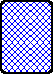
\includegraphics{card_back.pdf}};
	\pic[scale=0.095, transform shape] at (0,0) {head};

}}


\usepackage[hidelinks]{hyperref} % Add hyperlinks to the pdf file. This should usually be the last package loaded before \begin{document}

% Start Document

\begin{document}
% Cover page with title, cover art, description, and author
\center{\setmainfont{Charter}}
{\footnotesize{Version 0.1}}

\setmainfont[Scale=3.075, UprightFont={* 162 Bold}]{Libre Clarendon Normal}
{%\bfseries
\begin{center}
\begin{tabular}{@{}c@{\hspace{0.375ex}}l@{}c@{\hspace{0.425ex}}l@{}}
\Huge{H} & \Huge{\textcolor{red}{E}} & \Huge{A} & \Huge{\textcolor{red}{D}} \\[0.5ex]
\Huge{\textcolor{red}{T}} & \Huge{R} & \Huge{\textcolor{red}{I}} & \Huge{P}
\end{tabular}
\end{center}
}

\vfill

\setmainfont[Scale=1.5]{Charter}
\begin{center}
\LARGE
Headmaster's\phantom{y}Guide
\end{center}

\vfill

\begin{figure}[h]
\centering
	\begin{tikzpicture}
	\node (A) at (0,0) {
\includegraphics[scale=0.06]{head_outline.png}};
	\node (B) at (1.1,0.95) {\fontsize{60}{72}{\hearts}};
	\node (B) at (-1.9,0.95) {\fontsize{60}{72}{\diamonds}};
	\node (B) at (-0.475,2.6) {\fontsize{60}{72}{\spades}};
	\node (B) at (-0.475,-0.4) {\fontsize{60}{72}{\clubs}};
	\end{tikzpicture}
\end{figure}

\vfill

\setmainfont[Scale=1.5]{Charter}
\begin{center}
\LARGE
Michael\phantom{y}Purcell
\end{center}

\newpage

\setmainfont{Charter}
\raggedright
\section{Overview}
Head Trip, as described in the Player's Guide, is a competitive card game for four players.
In that version of the game, each player portrays one aspect of the personality of a teenage boy named Bobby.
These aspects compete with one another to control Bobby's actions as he faces a series of challenges.

The Headmaster's Guide describes an additional role for an additional player, the \emph{Headmaster}.
Rather than portraying an aspect of Bobby's personality, the Headmaster's job is to provide narrative context for everything that happens during the game.

This transforms Head Trip into a semi-cooperative roleplaying game in which the Headmaster helps the other players tell a story about Bobby's experiences.

These rules assume that the reader is familiar with the game described in the Player's Guide.

\section{The Cards}
In this version of the game, the players will use the \emph{Headmaster's deck} instead of the auxiliary deck described in the Player's Guide.
The Headmaster's deck is a complete (54-cards) standard deck of playing cards. It consists of:

\begin{auxiliarydecklist}
	\item[Challenge Cards\hfill\normalfont{(27):}] \two\ \textendash\ \ten\ of \clubs, \hearts, \spades.
	\item[Aspect Cards\hfill\normalfont{(4):}] \jack\clubs, \queen[red]\hearts[red], \king\spades, \ace[red]\diamonds[red].
	\item[Label Cards\hfill\normalfont{(3):}] \ace\clubs, \ace[red]\hearts, \ace\spades.
	\item[Location Cards\hfill\normalfont{(9):}] \redtwo\ \textendash\ \redten\ of \diamonds.
	\item[Character Cards\hfill\normalfont{(11):}] remaining \jack, \queen, \king, \joker\ cards.
\end{auxiliarydecklist} 

Notice that the challenge cards, aspect cards, and label cards are the same as those that comprise the auxiliary deck. The setting cards are not used in the game described in the Player's Guide.

So, this version of the game can still be played with two standard decks of playing cards. The Headmaster will use cards from the Headmaster's deck while the other players will use cards from the persona deck. 


\newpage
\subsection{Challenge Cards}
Each challenge card represents a challenge that Bobby faces during the game. Every challenge has both a type and a difficulty.

The type of a challenge represents the skills that Bobby will need to employ to successfully face that challenge. There are three types of challenge, each of which requires different skills:
\begin{challengetypelist}[itemsep=0pt]
	\item[\clubs\ (Physical):] requires athleticism or aggression. 
	\item[\hearts\ (Social):] requires empathy or insight.
	\item[\spades\ (Mental):] requires creativity or analysis.
\end{challengetypelist}

The difficulty of a challenge is represented by the rank of its challenge card. The higher the rank, the more difficult the challenge.

When Bobby faces a challenge, the pilot will play an action card. Bobby succeeds if the rank of that action card meets or exceeds that of the challenge card.

\subsection{Location Cards}

Each location card represents a place where Bobby might be found on a school day. With the exception of Bobby's House (where the story might begin or end) and the School Bus, all of these locations are different rooms in Bobby's school. 
\vspace{-1.75ex}
\begin{multicols}{2}
\begin{cardlist}[itemsep=0pt, topsep=0pt, partopsep=0pt]
  \item[\redtwo\diamonds:] Bobby's House
  \item[\redthree\diamonds:] School Bus
  \item[\redfour\diamonds:] Classroom
  \item[\redfive\diamonds:] Cafeteria
  \item[\redsix\diamonds:] Principal's Office
  \item[\redseven\diamonds:] Hallway
  \item[\redeight\diamonds:] Library
  \item[\rednine\diamonds:] Auditorium
  \item[\redten\diamonds:] Locker Room
  \item[]
\end{cardlist}
\end{multicols}

\subsection{Character Cards}
Each character card represents a person that Bobby might encounter at school. These include other kids, family members, school faculty, and other adults.
\vspace{-1.75ex}
\begin{multicols}{2}
\begin{cardlist}[itemsep=0pt, topsep=0pt, partopsep=0pt]
  \item[\redjack\diamonds:] Bully
  \item[\redqueen\diamonds:] Crush
  \item[\redking\diamonds:] Friend
  \item[\queen\clubs:] Neighbour
  \item[\king\clubs:] Janitor
  \item[\jack\spades:] Principal
  \item[\queen\spades:] Teacher
  \item[\redjack\hearts:] Sibling
  \item[\redking\hearts:] Parent
  \item[\hspace{0.19cm}\joker:] Stranger
\end{cardlist}
\end{multicols}

\newpage
\section{Game Play}
The game takes place over a sequence of rounds. During each round, the Headmaster should:
\begin{enumerate}
	\item Establish the setting for the current challenge. 
	\item Choose a challenge card for the pilot to reveal. The  other players will then elect a pilot. That pilot will then play an action card to the tableau.
	\item React to the action card played by the pilot.
\end{enumerate}

\subsection{Establishing the Setting}
The Headmaster should describe the location where the current challenge will take place and any non-player characters who might be involved.

The location cards and character cards can be used as a menu of possible setting elements that the Headmaster can choose from or as a way to generate random setting elements.

Each setting should present Bobby with a situation where the outcome  of the challenge is uncertain and where Bobby stands to benefit if he succeeds. 


\subsection{Choosing a Challenge Card}
The Headmaster should choose a challenge card appropriate for the setting of each challenge.

Challenge cards should not be reused.  Once Bobby has faced a challenge represented by a given challenge card, that card is unavailable for use in future challenges and should be discarded.
  

\subsection{Reacting to an Action Card}
The Headmaster should work with the pilot to describe how Bobby faces each challenge.

This description should incorporate the type and difficulty of the challenge, the rank of the pilot's action card, and whether Bobby succeeds or fails.

Bobby is always the one who is facing each challenge, not the pilot. The difference between the aspects is their motivations rather than their capabilities.


\newpage

\section{Sample Adventure}
The following is a series of challenges that the Headmaster can use as a starting point for their first story. The Headmaster should modify the challenges as necessary in response to the other players' actions.

\rule{\textwidth}{1pt}
\begin{description}[topsep=0pt, labelindent=0pt, leftmargin=0.0cm]	
	\item[Location 1\normalfont{:}] \redtwo\diamonds\ - Bobby's Bedroom
	\smallskip
	\begin{description}[labelindent = 0.5cm, leftmargin=0.75cm]
		\item[Challenge 1a\normalfont{:}] \three\clubs\ - Hit the snooze alarm and go back to sleep. Bobby's exhausted.
		\item[Challenge 1b\normalfont{:}] \redfour\hearts\ - Convince Bobby's mom that he won't be late for school. Again.
	\end{description}

	\rule{\textwidth}{1pt}

	\item[Location 2\normalfont{:}] \redthree\diamonds\ - Bus Stop
	\smallskip
	\begin{description}[labelindent = 0.5cm, leftmargin=0.75cm]
		\item[Challenge 2a\normalfont{:}] \five\spades\ - Figure out a shortcut that will let Bobby get to school on time. 
	\end{description}
	
	\rule{\textwidth}{1pt}
	
	\item[Location 3\normalfont{:}] \redfour\diamonds\ - Chemistry Class
	\smallskip
	\begin{description}[labelindent = 0.5cm, leftmargin=0.75cm]
		\item[Challenge 3a\normalfont{:}] \redfive\hearts\ - Meet the new girl. Her name is Annie. Try to make a good first impression.
	\end{description}
	
	\rule{\textwidth}{1pt}

	
	\item[Location 4\normalfont{:}] \redfive\diamonds\ - Cafeteria
	\smallskip
	\begin{description}[labelindent = 0.5cm, leftmargin=0.75cm]
		\item[Challenge 4a\normalfont{:}] \redeight\hearts\ - Bullies are picking on Annie in the lunch line. Ask them to leave her alone.
		\item[Challenge 4b\normalfont{:}] \six\clubs\ - The bullies pushed Bobby?!? That's it, this means war. Ramming speed! 
	\end{description}
	
	\rule{\textwidth}{1pt}
	
	\item[Location 5\normalfont{:}] \redsix\diamonds\ - Principal's Office
	\smallskip
	\begin{description}[labelindent = 0.5cm, leftmargin=0.75cm]
		\item[Challenge 5a\normalfont{:}] \seven\spades\ - The principal just asked Bobby what he thinks an appropriate punishment might be. Answer carefully.
	\end{description}
	
	\rule{\textwidth}{1pt}
	
	\item[Location 6\normalfont{:}] \redseven\diamonds\ - Hallway
	\smallskip
	\begin{description}[labelindent = 0.5cm, leftmargin=0.75cm]
		\item[Challenge 6a\normalfont{:}] \redten\hearts\ - Ask Annie to go out sometime after school. Maybe to the mall?
	\end{description}
	
	\rule{\textwidth}{1pt}

\end{description}
\medskip
None of the players are likely to have used all of their actions cards yet. The game (probably) isn't over! From here, the Headmaster should direct the story wherever the players seem to be most interested.

\newpage
\section{Variants}
Most of the rules of the game are independent of the setting elements. So, it is easy to modify the game to tell different kinds of stories.

\subsection{Other Settings}
Some players may want to explore Bobby's life outside of school. 

If the Headmaster is confident in their ability to improvise then they can simply invent new setting elements on the fly as required.

Otherwise, they can make their own lists of what the various location cards and character cards represent.

\subsection{Other People}
Some players may want to portray the aspects of the personality of someone other than Bobby.

In some cases, for example if the players want to play as aspects of Annie's personality, only names need to be changed and the setting elements can be left as is.

In other cases, the default setting won't make sense for the new person and the Headmaster will have to modify the setting accordingly.

\vfill

\section{Acknowledgements}
The design of Head Trip has been vastly improved by the influence of ideas and mechanics from other games and the feedback provided by playtesters throughout the design process.

The following tools were used to create this leaflet:
\begin{description}[labelindent = 0.25cm, itemsep=0pt, leftmargin=0.25cm]
	\item[Typesetting\normalfont{:}] XeLaTeX.
	\item[Diagrams\normalfont{:}] TikZ, GIMP.
	\item[Fonts\normalfont{:}] Libre Clarendon, Charter, Card~Characters.
\end{description}

\medskip

\textbf{Contact}: \href{mailto:head.trip.card.game@gmail.com}{head.trip.card.game@gmail.com}

\smallskip

\begin{tabular}{@{}m{\textwidth-\widthof{\Huge{\doclicenseIcon}}}@{}m{\widthof{\Huge{\doclicenseIcon}}}@{}}
\footnotesize{This work is licensed under a Creative Commons\newline ``Attribute 4.0 International'' license.} & \Huge{\doclicenseIcon} \\
\end{tabular}
\end{document}